\usetikzlibrary{decorations.fractals}

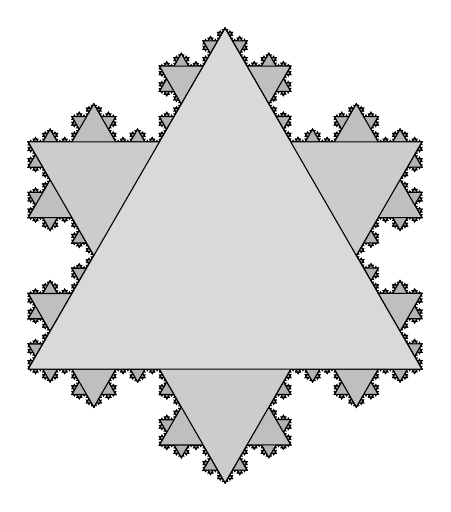
\begin{tikzpicture}[decoration=Koch snowflake,scale=5/3]
    \draw[fill=gray!90] decorate{ decorate{ decorate{ decorate{ decorate{
       (0,0) -- ++(60:3)  -- ++(300:3) -- ++(180:3)}}}}};
    \draw[fill=gray!80] decorate{ decorate{ decorate{ decorate{
       (0,0) -- ++(60:3)  -- ++(300:3) -- ++(180:3)}}}};
    \draw[fill=gray!60] decorate{ decorate{ decorate{
       (0,0) -- ++(60:3)  -- ++(300:3) -- ++(180:3)}}};
    \draw[fill=gray!50] decorate{ decorate{
       (0,0) -- ++(60:3)  -- ++(300:3) -- ++(180:3)}};
    \draw[fill=gray!40] decorate{
       (0,0) -- ++(60:3)  -- ++(300:3) -- ++(180:3)};
    \draw[fill=gray!30] (0,0) -- ++(60:3)  -- ++(300:3) -- ++(180:3);
\end{tikzpicture}
\caption{
Der Inhalt der sogenannten Koch-Schneeflocke besteht aus einer unendlichen Anzahl Dreiecke. Die Seiten der kleineren Dreiecke entsprechen stets einem Drittel der grösseren Seiten. Die Fläche eines Dreiecks nimmt also in jedem Schritt um den Faktor $\frac{1}{9}$ ab. Um die Gesamtfläche der ganzen Schneeflocke zu bestimmen, muss man die unendliche geometrische Reihe berechnen:
\[ 1 + 3(\frac{1}{9}) + 12 (\frac{1}{9})^{2} + 48 (\frac{1}{9})^{3}... \] 
Die Reihe konvergiert, damit ist die Fläche endlich, wird jedoch von einer unendlich langen Strecke umschlossen.
}
%https://en.wikipedia.org/wiki/Geometric_series
